\chapter{Einführung}\label{ch:intro}

Das Smartphone ist heutzutage der stete Begleiter eines Menschen. \enquote{Zwei Drittel der Bevölkerung und nahezu jeder 14- bis 29-Jährige geht darüber ins Netz.} \cite{usage} Auch die Prognose zeigt, das der Absatzmarkt immer weiter steigen wird (Abbildung \ref{fig:prognose_fig}).

\begin{figure}[H]
	\begin{center}
		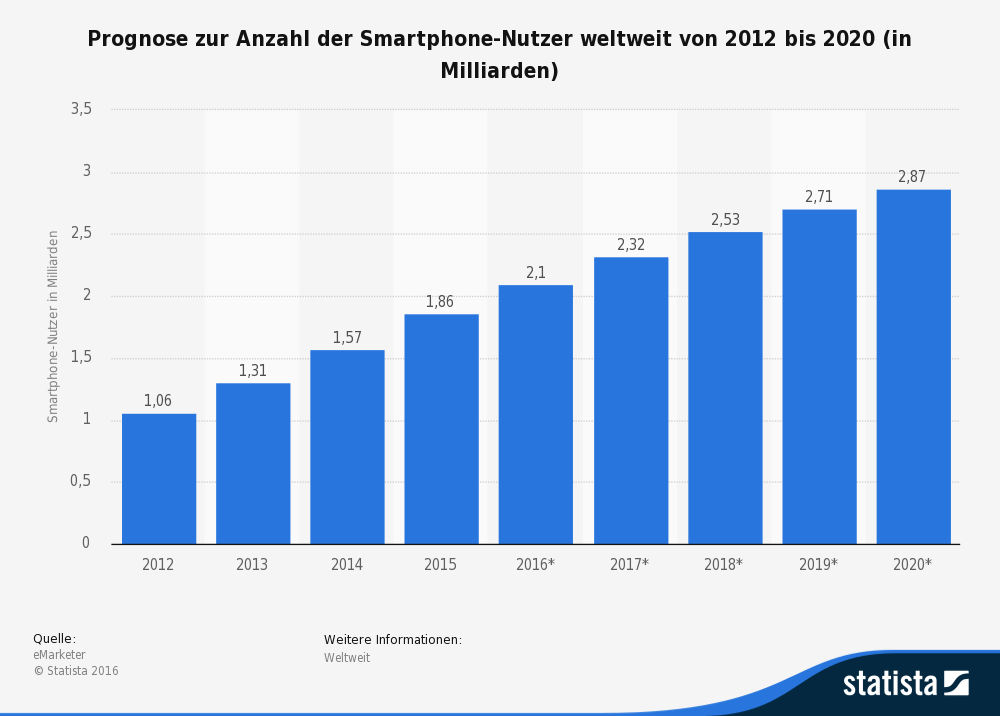
\includegraphics[width=0.86\textwidth]{images/prognose-zur-anzahl-der-smartphone-nutzer-weltweit-bis-2020.png}
		\caption{Prognose zur Anzahl der Smartphone-Nutzer weltweit von 2012 bis 2020 (in Milliarden) \cite{prognose}.}
		\label{fig:prognose_fig}
	\end{center}
\end{figure}

Umso wichtiger ist es das die Softwareentwicklung diesen Trend ernst nimmt. Der ehemalige Google-Chef Eric Schmidt sagte bereits 2010: \enquote{Googles Devise heißt jetzt \enquote{Mobile first}}. 
Diese Devise wird von vielen Unternehmen verfolgt, das ist der Grund weswegen in den einzelnen Stores heutzutage so viele Apps angeboten werden. Bei Android im Playstore sind es im Oktober 2016 ca. 2,4 Millionen Apps \cite{play_store}, bei Apple im App Store sind es ca. 2 Millionen Apps (Stand Juni 2016) \cite{app_store}. Neben Googles Android und Apples iOs gibt es noch andere Betriebssysteme, beispielsweise Microsofts Windows Phone oder Blackberrys Blackberrys OS. Jedoch bestimmen die beiden erstgenannten Systeme den Markt (Abbildung \ref{fig:os_fig}).

\begin{figure}[H]
	\begin{center}
		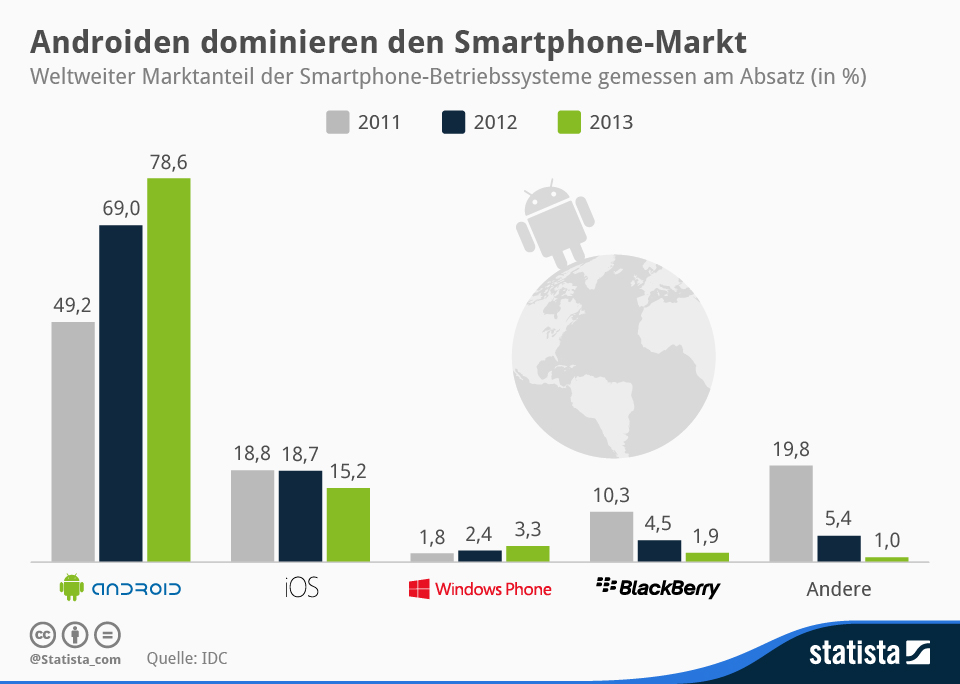
\includegraphics[width=0.86\textwidth]{images/os.jpg}
		\caption{Der weltweite Marktanteil von Smartphone-Betriebssysteme \cite{os}.}
		\label{fig:os_fig}
	\end{center}
\end{figure}

Jede dieser Applikationen wurden einzeln für sich entwickelt und implementiert. Bei jedem Update zum Beispiel des Systems, müssen alle Anwendungen gewartet und überarbeitet werden, um die volle Funktionalität zu gewährleisten.

Würden einige Applikationen jedoch genauer analysiert werden, wäre das Ergebnis, dass in jeder dieser Anwendungen Codepassagen vorhanden sind, welche einen ähnlichen beziehungsweise den selben Zweck erfüllen. Werden diese Stellen im Programmcode abstrahiert, gibt es die Möglichkeit diese generieren zu lassen. Um Code generieren zu lassen, benötigt man so genannte Code-Generatoren. 

Im Bereich der Backend-Entwicklung gibt es bereits verschiedene Projekte die sich damit befassen. Ein Beispiel wäre der \textit{CRUD Admin Generator} \cite{generators}. Die Hochschule für angewandte Wissenschaften Würzburg-Schweinfurt entwickelt  unter der Leitung von Prof. Dr. Peter Braun auch einen Code-Generator unter dem Namen: \ac{gemara}. Mit Hilfe solcher Generatoren für den Bereich von Mobilen Applikationen, könnte der Entwicklungs- und Wartungsaufwand reduziert werden. 

Führt ein Systemupdate dazu, dass die Implementierung von verschiedenen Anforderungen nicht weiter funktionsfähig ist, muss dies nur einmalig an der entsprechenden Stelle im Code-Generator geändert werden und nicht in jeder Applikation einzeln. 

\section{Motivation}\label{sec:motivation}
Im Rahmen des Projektes \ac{gemara} gab es bereits Arbeiten, welche sich mit dem Thema der Generierung von \textit{Android Aktivities} beschäftigt. Die dabei entstandenen Lösungen, resultieren darin, das dass generieren von \textit{Aktivities} zu Problemen führt. Deshalb beschäftigt sich diese Ausarbeitung damit, nicht eine komplette \textit{Aktivity} zu erzeugen, sondern sogenannte Komponenten.

Eine Komponente, ist im wesentlichen eine kleine Anwendung für sich, welche nur eine einzige Aufgabe erfüllt. Dies könnte zum Beispiel das Anzeigen eines Dozenten in einer Campus-Applikation sein.
Aus den erzeugten Komponenten, kann eine Art Bausatz entstehen. Mit dessen Hilfe der Entwickler seine Applikation zusammen bauen kann. Dabei wird ihm freie Wahl gelassen, wie der Aufbau seiner Anwendung aussieht, er bedient sich nur an gegebener Stelle an den Komponenten. Dadurch reduziert sich der Entwicklungsaufwand für ihn.

Bewegen wir uns in der Domain einer Hochschule, so kann eine Bibliothek mit den erzeugten Komponenten allen Studierenden zur Verfügung gestellt werden. Dadurch wäre jeder dieser Studierenden in der Lage eine persönliche Campus-Applikation zu entwickeln. Durch die einzelnen Komponenten kann dann sichergestellt werden, dass grundsätzliche Funktionalität bereits gewährleistet ist.

\section{Zielsetzung}\label{sec:target}
Ziel dieser Ausarbeitung liegt darin, dass der Leser ein grundsätzliches Verständnis für die Entwicklung von Android Applikationen beziehungsweise Android-Bibliotheken vermittelt bekommt. Weiterhin soll das Wissen über Datenkommunikation mittels \textit{\ac{rest}} vertieft werden. Hierbei wird ein Schwerpunkt auf das \textit{Hypermedia-Prinzip} gelegt. 

Neben diesen spezifischen Anforderungen, soll ein Verständnis für der Implementierung von Generatoren entstehen. Dafür muss der Entwickler entscheiden können, was von der Implementierung als statischer Code angesehen werden kann und welcher generisch ist. Dieses Verständnis ist wichtig, um die Komplexität der Generatoren zu reduzieren. Da die statischen Anteile jedes mal identisch sind.
Auch soll auf die Frage eingegangen werden, ob man das \textit{\ac{ui}}, welches ebenfalls generiert wird, auch generisch gestalten kann. Das bedeutet, dass nicht nur die Informationen, welche angezeigt werden sollen beschreibt. Sondern auch wie diese angezeigt werden sollen.

Wenn es möglich ist dass das \textit{\ac{ui}} als Teil der \textit{\acf{dsl}} beschrieben werden kann, so hat der Nutzer des entsprechenden Generators die Freiheit, selbst zu entscheiden ob zum Beispiel bei seiner Campus-App, bei der Liste aller Dozenten das Profilbild links oder rechts angezeigt werden soll.

\section{Aufbau der Arbeit}\label{sec:structure}
Diese Ausarbeitung ist in sieben Kapitel unterteilt. In der Einführung wird zu Beginn auf den Stellenwert von Android Applikationen eingegangen. Darauf folgt die Motivation, weswegen diese Arbeit geschrieben wurde. Diese soll die Problemstellung anreißen und zur Zielsetzung hinführen. In diesem Teil der Einführung wird definiert, was der Sinn dieser Arbeit ist. Das Kapitel wird dann mit dem Bereich abgeschlossen, welchen den Aufbau der Arbeit beschreibt.

Das zweite Kapitel befasst sich mit den Grundlagen. Hier soll der Leser noch einmal seinen Kenntnisstand über \textit{\acf{rest}} auffrischen und die Bedeutung von \textit{\acf{hateoas}} verstehen. Neben dem Bereich der Netzwerkkommunikation wird außerdem noch der Bereich Android angeschnitten. Hier liegt der Schwerpunkt in der Entwicklung und \textit{CustomViews}. Dabei werden die einzelnen Schritte aufgezeigt, die benötigt werden um diese Komponenten zu erstellen und zu benutzen. Der letzte Teil in den Grundlagen befasst sich mit Software-Generatoren. Hier wird dem Leser kurz erklärt was eine \textit{\acf{dsl}} ist und welche zwei generelle Arten es gibt.
Zum Anschluss wird das Projekt \acf{gemara} vorgestellt. 

Im folgenden Kapitel wird die Problemstellung behandelt, dabei wird die Referenzanwendung vorgestellt. Diese Vorstellung inkludiert sowohl das Backend sowie die Android Applikation. Es wird darauf eingegangen das das Backend mit Hilfe von \ac{gemara} generiert wurde und wie das daraus resultierende \acl{api} aussieht. Anschließend wird die Anwendung dahingehend analysiert, dass eine Einteilung in generischen sowie spezifischen Quellcode vorgenommen werden kann. Auch werden die einzelnen \textit{Views} analysiert. Diese Analyse sollen Gemeinsamkeiten beim Aufbau und Design offenbaren. So das diese mit einer \textit{\ac{dsl}} beschrieben werden können. Zum Abschluss wird das \textit{Meta-Modell} vorgestellt. Es wird auf die Anforderungen an dieses eingegangen und anschließend zwei Modelle vorgestellt. Ein reines Android Modell und dann die Erweiterung des vorhandenen Enfield-Modells. Der nächste Bereich befasst sich mit der Analyse, hierbei soll herausgefunden werden welche Daten das \textit{Meta-Modell} überhaupt benötigt. In der Analyse werden die einzelnen \textit{Views} genauer betrachtet und es wird ein Augenmerk auf den Programmablauf und die Aktionen bei Klick gelegt. Nach der Analyse wird der Aufbau der \textit{View-Meta-Modelle} vorgestellt. Bei jeder \textit{View} wird auf deren Besonderheit und Möglichkeiten eingegangen. Neben den \textit{View-spezifischen} Daten wird auch noch aufgezeigt, welche Dateien allgemein benötigt werden und wo diese im vorgegebenen Modell platziert werden sollten. 

Das Kapitel Lösung stellt \textit{Welling} vor. Dies ist der in dieser Arbeit entwickelte Software-Generator. Zunächst wird das \textit{Java \acf{api} JavaPoet} im Zusammenhang mit der Generierung von Java-Klassen vorgestellt, anschießend wird beschrieben, wie andere Datei-Typen generiert werden können. Es wird gezeigt welche Features unterstützt werden müssen. Nachfolgend wird der Aufbau des Generators vorgestellt. Es wird auf die einzelnen Bereiche eingegangen und deren Aufgabe sowie Funktionsweise erklärt. Abgeschlossen wird das Kapitel mit einer Anleitung, wie die generierte Applikation gebaut und ausgeführt werden kann.

Das fünfte Kapitel, Evaluierung anhand einer Beispielanwendung, ist in drei Bereiche eingeteilt. Am Anfang wird die Beispielanwendung vorgestellt. Anschließend wird auf die Erstellung und Nutzung des \textit{Meta-Modells} eingegangen, wobei hier auch Einschränkungen durch dieses aufgezeigt werden. Der letzte Bereich befasst sich dann noch einmal mit den Zeitaufwänden und der Komplexität der Entwicklung, Wartung und Nutzung des Generators. Auch wird die Komplexität der erzeugen Applikation kritisch bewertet.

Im letzten Kapitel, Zusammenfassung, wird die Arbeit noch einmal Revue passieren lassen. Zusätzlich noch mögliche Erweiterungen und Ergänzungen an \textit{Meta-Modell} und Software-Generator vorgestellt.